% Created 2018-09-17 Mon 00:01
% Intended LaTeX compiler: pdflatex
\documentclass[presentation]{beamer}
\usepackage[utf8]{inputenc}
\usepackage[T1]{fontenc}
\usepackage{graphicx}
\usepackage{grffile}
\usepackage{longtable}
\usepackage{wrapfig}
\usepackage{rotating}
\usepackage[normalem]{ulem}
\usepackage{amsmath}
\usepackage{textcomp}
\usepackage{amssymb}
\usepackage{capt-of}
\usepackage{natbib}
\usepackage[linktocpage,pdfstartview=FitH,colorlinks,
linkcolor=blue,anchorcolor=blue,
citecolor=blue,filecolor=blue,menucolor=blue,urlcolor=blue]{hyperref}
\setbeamertemplate{frame footer}{\insertshortauthor}
\setbeamerfont{page number in head/foot}{size=\tiny}
\setbeamercolor{footline}{fg=gray}
\author{Florian Hollenbach}
\usepackage[english]{isodate}
\usepackage{amsmath,amsthm,amssymb,amsfonts}
\usetheme{metropolis}
\usecolortheme{}
\usefonttheme{}
\useinnertheme{}
\useoutertheme{}
\author{Florian Hollenbach}
\date{\today}
\title{Political Science 209 - Fall 2018}
\subtitle{Observational Studies}

\hypersetup{
 pdfauthor={Florian Hollenbach},
 pdftitle={Political Science 209 - Fall 2018},
 pdfkeywords={},
 pdfsubject={},
 pdfcreator={Emacs 25.3.1 (Org mode 9.1.9)}, 
 pdflang={English}}
\begin{document}

\maketitle


\begin{frame}[label={sec:org6a89c07}]{Review}
\begin{block}{What is the fundamental problem of causal inference?}
\end{block}
\end{frame}

\begin{frame}[label={sec:org258466d}]{Review}
\begin{block}{What about randomized control trials allows us to credibly estimate a causal effect?}
\end{block}
\end{frame}

\begin{frame}[label={sec:org4dbd159}]{Get out the Vote Study}
\begin{block}{What can induce citizens to vote?}
\end{block}
\end{frame}

\begin{frame}[label={sec:orgf19daca}]{What was the experiment?}
\pause
Letters to randomized households with treatment:
\begin{enumerate}
\item Naming and Shaming: your neighbors will know
\item Civic Duty
\item Hawthorne Effect Message
\item Control (no letter)
\end{enumerate}
\end{frame}

\begin{frame}[label={sec:orga0ff1c2}]{Let's go to R-studio quick}
\end{frame}


\begin{frame}[label={sec:org8fabebf}]{Observational Studies and Causal Inference}
\begin{block}{What is the main problem for observational studies?}
\pause
\begin{itemize}
\item Confounders: variables that are associated with both treatment and outcome
\end{itemize}
\end{block}
\end{frame}

\begin{frame}[label={sec:org3e9d156}]{What is the Problem with Confounders?}
\pause

\begin{itemize}
\item If pre-treatment characteristics are associated with treatment and outcome, we can't disentangle causal effect from confounding bias
\end{itemize}

\pause

\begin{itemize}
\item Selection into treament example: Maybe minimum wage was increased because unemployment was particularly low in NJ, but not PA
\end{itemize}
\end{frame}

\begin{frame}[label={sec:orgd6f8a1d}]{Examples of Confounding}
\begin{itemize}
\item Are incumbents more likely to win elections? Yes, but\ldots{}
\end{itemize}

\pause

\begin{itemize}
\item Incumbents receive more campaign contributions
\item Incumbents have more staff
\end{itemize}
\end{frame}

\begin{frame}[label={sec:org6a56cc6}]{Examples of Confounding}
\begin{itemize}
\item Does higher income lead countries to democratize?
\end{itemize}

\pause

\begin{itemize}
\item Higher income countries have more educated populations
\end{itemize}
\end{frame}



\begin{frame}[label={sec:orgca35130}]{What can we do about confounding in observational studies?}
\pause

\begin{itemize}
\item Make \emph{Treatment} and \emph{Control} groups as similar to each other as possible
\item Especially on variables that might matter for treatment status and outcome
\item Analyze subsets or \emph{statistical control}, such that we compare treated and control units that have same value on confounder
\end{itemize}
\end{frame}

\begin{frame}[label={sec:org3af8b70}]{Another problem with observational studies:}
\begin{itemize}
\item Reverse causality
\end{itemize}

\pause

\begin{itemize}
\item Example: Does economic growth cause democratization or democratization cause growth?
\end{itemize}

Why do experiments not suffer from the threat of reverse causality?
\end{frame}

\begin{frame}[label={sec:org7bb327e}]{Observational studies}
Difference-in-Differences Design
\end{frame}

\begin{frame}[label={sec:org44bb42c}]{Difference-in-Differences Design}
\begin{itemize}
\item Compare trends before and after the treatment across the same units
\item Takes initial conditions into account
\end{itemize}
\end{frame}

\begin{frame}[label={sec:orge1f39a1}]{Difference-in-Differences Design}
\begin{itemize}
\item Need data measured for both treatment and control at two different time periods: before and after treatment
\end{itemize}
\begin{center}
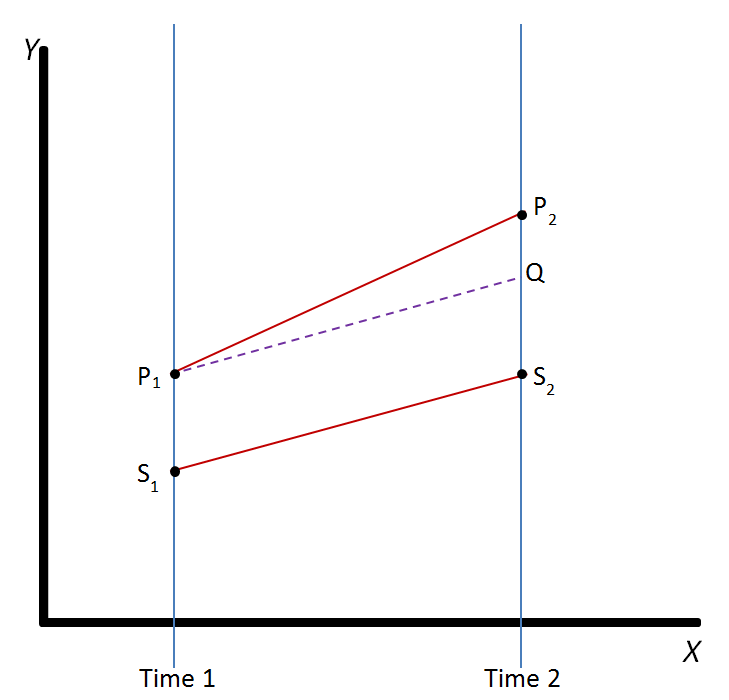
\includegraphics[width=4cm]{/Users/florianhollenbach/Documents/GitHub/Polisci209_2018/slides/week3/Illustration_of_Difference_in_Differences.png}
\end{center}

\begin{itemize}
\item Total difference between P2 and S2 can not be attributed to treatment. Why?
\end{itemize}
\end{frame}

\begin{frame}[label={sec:org2992c7a}]{Difference-in-Differences Design}
\begin{center}
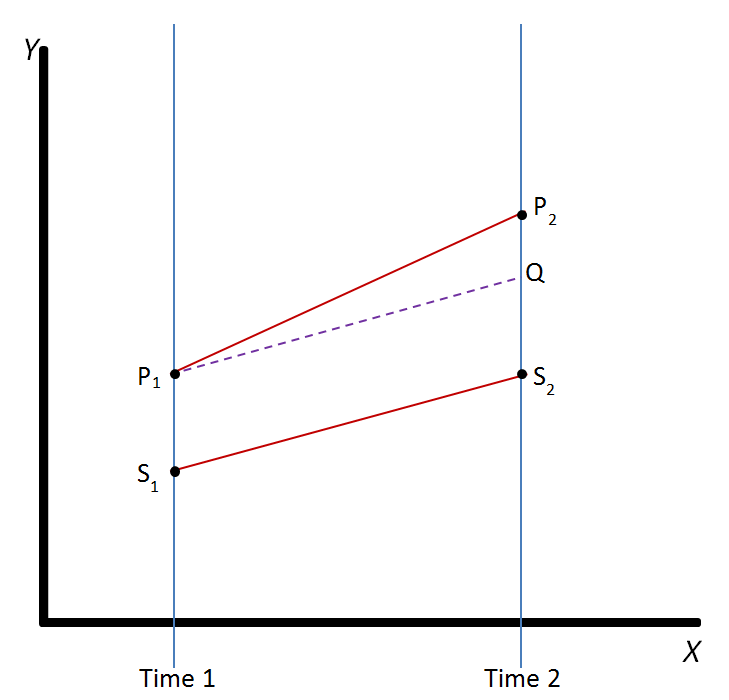
\includegraphics[width=4cm]{/Users/florianhollenbach/Documents/GitHub/Polisci209_2018/slides/week3/Illustration_of_Difference_in_Differences.png}
\end{center}

What might be a necessary condition for Diff-in-Diff to work?

\pause

Parralel Trends Assumptions
\end{frame}

\begin{frame}[label={sec:org82fba56}]{Difference-in-Differences Design}
\begin{center}
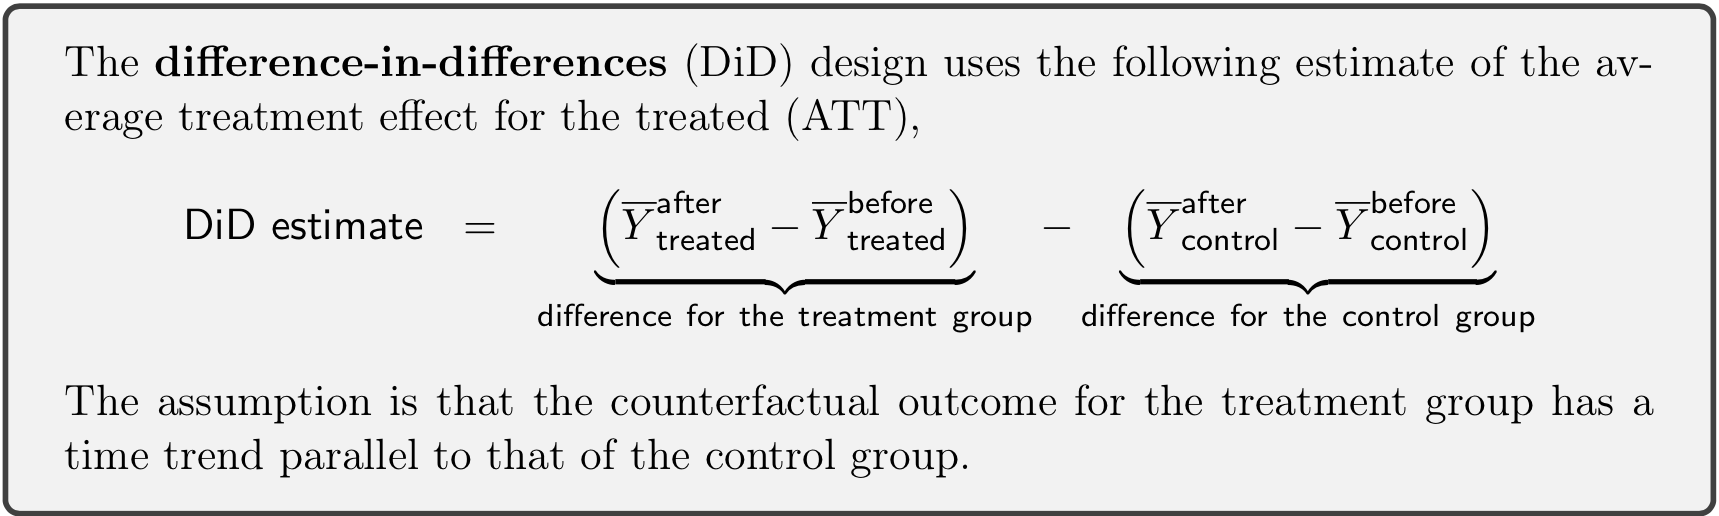
\includegraphics[width=8cm]{/Users/florianhollenbach/Documents/GitHub/Polisci209_2018/slides/week3/did.png}
\end{center}
\end{frame}


\begin{frame}[label={sec:org8776b3d}]{Describing numeric variables:}
\begin{itemize}
\item Mean
\item Median
\item Quantiles
\end{itemize}
\end{frame}


\begin{frame}[label={sec:orge62e587}]{Quantiles}
\begin{itemize}
\item splitting observations into equaly size groups, e.g., quartiles, quantiles
\item 75th percentile is the threshold under which 75\% of observations lie
\item What percentile is the median?
\end{itemize}
\end{frame}


\begin{frame}[label={sec:org783f3bf}]{Describing the spread of numeric variables:}
\begin{itemize}
\item IQR:
\end{itemize}

\pause

Difference between 75th percentile and 25th percentile
\end{frame}

\begin{frame}[label={sec:org506d3ca}]{Describing the spread of numeric variables:}
Standard Deviation

\pause


SD = \(\sqrt{\frac{1}{n} \sum^{N}_{i = 1} (x_{i} - \bar{x})^{2}}\)
\end{frame}

\begin{frame}[label={sec:orgc43fe32}]{Standard Deviation}
\begin{center}
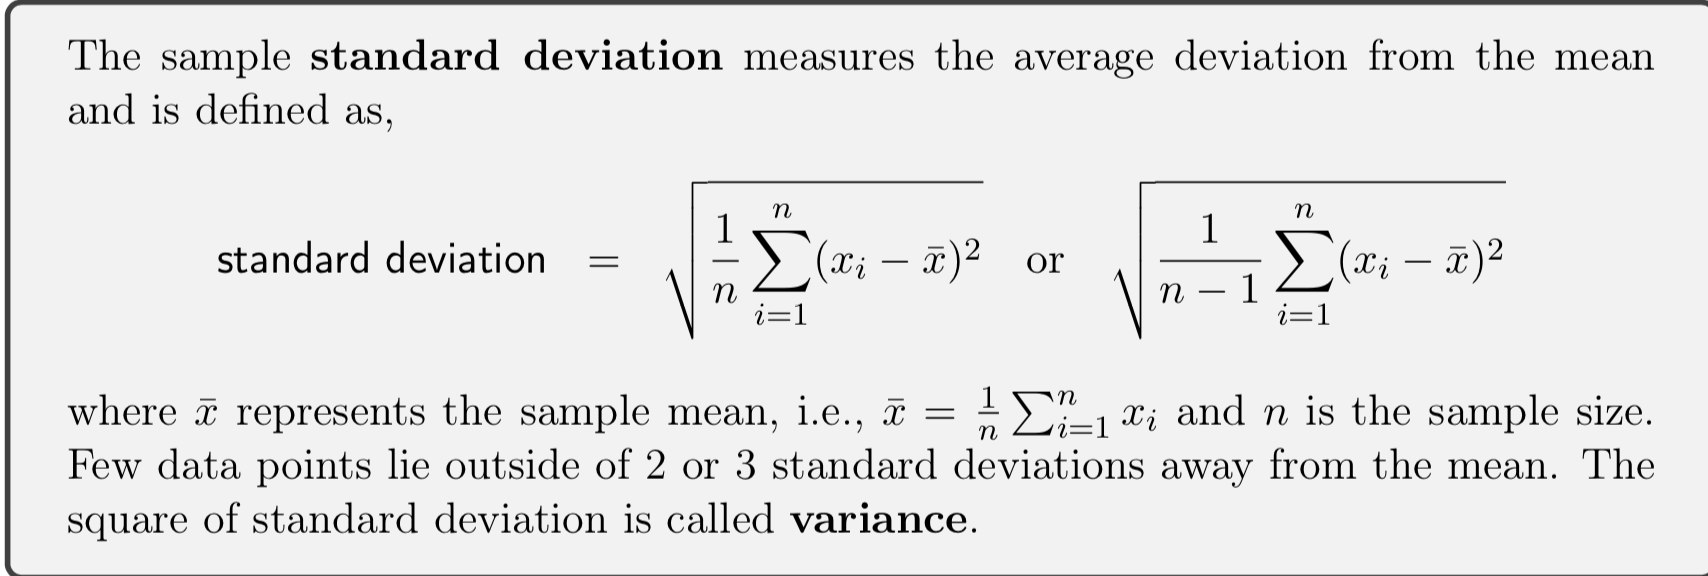
\includegraphics[width=8cm]{/Users/florianhollenbach/Documents/GitHub/Polisci209_2018/slides/week3/sd.png}
\end{center}
\end{frame}
\end{document}